\Chapter{Egy étterem, több futár, több kiszállítás esete}

\Section{A probléma megfoglmazása}

Jelen eset reprezentálja az egy lerakatos több ügynökös utazó ügynök problémát. A feltételek meghatározásánál nélkülözhetetlen szempont, hogy határokat szabjunk az egyes futároknak, hogy ki milyen területre szállít ki. Ennek meghatározásánál fontos a kiszállítási címek közti táv figyelembe vétele. Ezek meghatározása után maga a probléma leegyszerűsíthető egy klasszikus utazó ügynök problémára.
A probléma egy szemléltetését láthatjuk \aref{fig:model4}. ábrán.

\begin{figure}[h!]
\centering
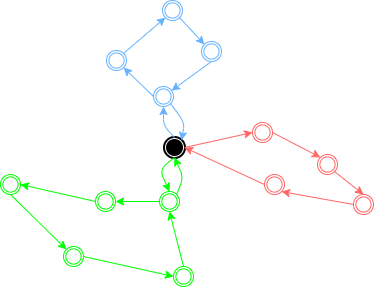
\includegraphics[scale=0.7]{images/Onedepotmtsp.png}
\caption{Egy étterem, több futár, több kiszállítás modellje}
\label{fig:model4}
\end{figure}

\Section{A probléma megoldása}

A több ügynökös, egy lerakatos utazó ügynök probléma modellje kiszállítási helyzetekre szabva írható le.

A több ügynökös, egy lerakatos utazó ügynök probléma esetén legyen $V$ a csúcsok halmaza, $x_{i,j}$ az, hogy megy-e az $i.$ pontból út a $j.$ pontba közvetlenül, $d_{i.j}$ az $i.$ és $j.$ pont távolsága. Legyen $m$ az ügynökök száma. Ezáltal a kapott célfüggvény:
\[
\displaystyle
\min \sum_{i=0}^n \sum_{j=0}^n d_{i,j} x_{i,j}.
\]
Minden pontba csakis egy út indul, kivétel ez alól a 0. pont ami maga az étterem:
\[
\displaystyle
\sum_{i=1}^n x_{i,j} = 1, \quad j = 1, 2, \ldots, n, i \neq j.
\]

Minden pontból csak egy út érkezik, kivétel ez alól a 0. pont ami maga az étterem:
\[
\displaystyle
\sum_{j=1}^n x_{i,j} = 1, \quad i = 1, 2, \ldots, n, i \neq j.
\]

Az étteremre vonatkozó feltétel:
\[
\displaystyle
\sum_{i=1}^n x_{i, 0} = m, \quad
\sum_{j=1}^n x_{j, 0} = m.
\]

MTSP esetén a kövezkező megszorítások szükségesek:
\[
u_i - u_j + p x_{i,j} \leq p - 1, \quad i, j = 1, 2, \ldots, n, i \neq j,
\]
továbbá
\[
\displaystyle
\sum_{i \notin S} \sum_{j \notin S} x_{i,j} \geq r(S), \quad
\forall S \subseteq V \setminus \{0\}, S \neq \emptyset,
\]
ahol $S$ a pontok egy részhalmaza, $r(S)$ pedig az, hogy ezt a részhalmazt minimum hány futárnak kell látogatnia. A definíció szumma része megmutatja, hogy minimum hány út megy be a vizsgált pontba. Az éttermet figyelmen kívűl hagyjuk $m$ darab út hagyja el és $m$ darab út megy ki belőle. Ezáltal a fenti egyenlőtlenség nem a futárok tényleges számát adná vissza.

Magát a problémát genetikus algoritmussal oldottam meg. A következő szakaszban ennek részletezésére kerül sor.

\Section{Megoldás genetikus algoritmus segítségével}

A genetikus algoritmust számítógépes szimulációkkal reprezentálják. A keresési teret egyedek populációi alkotják. Ezen egyedeket lehet keresztezni (más szóval rekombinálni) és mutálni is, ezáltal új egyedek kreálhatóak. Fitnesz függvénynek nevezzük a keresési téren értelmezett célfüggvényt. Az algoritmus működése során új egyedeket képes létrehozni a rekombinációs és mutációs operátorokkal, valamint kiszűri a rosszabb fitnesz függvény értékkel rendelkező egyedeket, majd ezt követően kiszedi azokat a populációból.

Az algoritmus működésének a folyamata a következő lépésekben foglalható össze.

1. \textit{Inicializáció}:  Az induló populációt legkönnyebben véletlenszerű számokkal tudjuk létrehozni. Maga a populáció mérete erősen függ a problémától. A keresési térben az egyedek általában egyenletesen oszlanak el, viszont számos esetben több egyedet generál a feltételezhető optimum közelében. \\

2. \textit{Kiválasztás}: Az összes eredményes generációban szelekcióra kerül az aktuális populáció egy része szaporodásra. A kiválasztás rendszerint fitnesz alapján történik, ahol a fitnesz függvény szerinti legfitebb egyedek valószínűbben kerülnek szelekcióra. Számos metódus az összes egyed fitneszét figyelembe veszi és ezek alapján keresi a legjobbat. Akadnak olyan metódusok is amik csak néhány véletlenszerűen kiválasztott példányt vizsgálnak. A példány minőségének mérésére használják a fitnesz függvényt. Ezen függvény bonyolultsága minden esetben a problémától függ. \\

3. \textit{Szaporítás}: Egyoperandusú mutációval valamint kétoperandusú keresztezési műveletek által lehetséges a példányokból újabb példányokat kreálni. Ezen operátorokat véletlenszerűen használják. \\

4. \textit{Leállás}: A genetikus algoritmus addig fut amíg be nem teljesül a leállási feltétel.\\

A módszer előnye: Kedvező eredménnyel használható majdnem minden problémára. Folytonos, illetve diszkrét problémáknál úgyszintén alkalmazható. A folyamatok könnyen páhuzamosíthatóak általa.

Hátránya: A megfelelő operátor kiválasztása nehéz. Paraméterezése és a leállási feltétel meghatározása sok időt igényel, valamint nem garantált a globális optimum elérése.

Elitizmus: Ebben az esetben a jelenlegi populáció legjobb egyedét mindig, módosítás nélkül visszük tovább az új populációba.

\Section{A megoldás implementálása}

A genetikus algoritmus megvalósítása a \texttt{dustbin} modul \texttt{Dustbin} nevű osztálya, és a \texttt{galogic} modul \texttt{GA} nevű osztálya segítségével történt.
Ezekhez hozzá tartoznak még a \texttt{main}, \texttt{globals}, \texttt{population}, \texttt{route} és a \texttt{routeManager} nevű modulok.
A következőkben ezek bemutatására kerül sor.

\subsection{A \texttt{Dustbin} osztály}

A \texttt{Dustbin} osztály reprezentálja a bejárható pontokat az útvonalban, annak $x$ és $y$ koordinátájával (\ref{fig:dustbin}. ábra).

\begin{figure}[!htb]
\centering
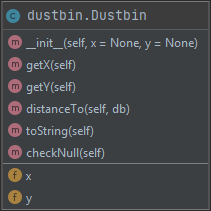
\includegraphics[scale=0.7]{images/dustbin.png}
\caption{Dustbin osztály metódusai és adattagjai}
\label{fig:dustbin}
\end{figure}

Inicializáló metóduson kívűl található benne még olyan folyamat ami felel, az $x$ és $y$ értékek feldolgozásával. Ezen felül az euklidészi távolság számítás is itt foglal helyet. Továbbá található még benne egy formázó metódus, ami a szöveget helyesen formázottan adja vissza.

\subsection{A \texttt{galogical} modul}

Az eljárás lényegi, logikai része a \texttt{GA} osztályban valósul meg (\ref{fig:galogical}. ábra).

\begin{figure}[!htb]
\centering
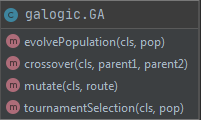
\includegraphics[scale=0.8]{images/galogic.png}
\caption{Galogical osztály metódusai}
\label{fig:galogical}
\end{figure}

Az \texttt{evolvePopulation} a populáció fejlesztésére használt metódus. Tartalmaz egy ellenőrzést, hogy kívánunk-e elitizmussal élni a futás alatt vagy sem. Ezenfelül a keresztezés és mutáció operátorokat meghívó programkódok is itt foglalnak helyet.

\begin{python}
@classmethod
def evolvePopulation(cls, pop):

    newPopulation = Population(pop.populationSize, False)

    elitismOffset = 0
    if elitism:
        newPopulation.saveRoute(0, pop.getFittest())
        elitismOffset = 1

    for i in range(elitismOffset, newPopulation.populationSize):
        parent1 = cls.tournamentSelection(pop)
        parent2 = cls.tournamentSelection(pop)
        child = cls.crossover(parent1, parent2)
        newPopulation.saveRoute(i, child)

    for i in range(elitismOffset, newPopulation.populationSize):
        cls.mutate(newPopulation.getRoute(i))

    return newPopulation
\end{python}

A keresztezési operátor implementációját a következő metódussal oldottam meg.
\begin{python}
@classmethod
def crossover(cls, parent1, parent2):
    child = Route()
    child.base.append(Dustbin(-1, -1))
    startPos = 0
    endPos = 0
    while startPos >= endPos:
        startPos = random.randint(1, numNodes - 1)
        endPos = random.randint(1, numNodes - 1)

    parent1.base = [parent1.route[0][0]]
    parent2.base = [parent2.route[0][0]]

    for i in range(numDeliverer):
        for j in range(1, parent1.routeLengths[i]):
            parent1.base.append(parent1.route[i][j])

    for i in range(numDeliverer):
        for j in range(1, parent2.routeLengths[i]):
            parent2.base.append(parent2.route[i][j])

    for i in range(1, numNodes):
        if i > startPos and i < endPos:
            child.base[i] = parent1.base[i]

    for i in range(numNodes):
        if not(child.containsDustbin(parent2.base[i])):
            for i1 in range(numNodes):
                if child.base[i1].checkNull():
                    child.base[i1] =  parent2.base[i]
                    break

    k = 0
    child.base.pop(0)
    for i in range(numDeliverer):
        child.route[i].append(RouteManager.getDustbin(0))
        for j in range(child.routeLengths[i]-1):
            child.route[i].append(child.base[k])
            k += 1
    return child
\end{python}

A mutáció operátor kódja az alábbi.
\begin{python}
@classmethod
def mutate (cls, route):
    index1 = 0
    index2 = 0
    while index1 == index2:
        index1 = random.randint(0, numDeliverer - 1)
        index2 = random.randint(0, numDeliverer - 1)

    route1startPos = 0
    route1lastPos = 0
    while route1startPos >= route1lastPos or route1startPos == 1:
        route1startPos =
          random.randint(1, route.routeLengths[index1] - 1)
        route1lastPos =
          random.randint(1, route.routeLengths[index1] - 1)

    route2startPos = 0
    route2lastPos = 0
    while route2startPos >= route2lastPos or route2startPos == 1:
        route2startPos =
          random.randint(1, route.routeLengths[index2] - 1)
        route2lastPos= random.randint(1, route.routeLengths[index2] - 1)

    swap1 = []
    swap2 = [] 

    if random.randrange(1) < mutationRate:
        for i in range(route1startPos, route1lastPos + 1):
            swap1.append(route.route[index1].pop(route1startPos))

        for i in range(route2startPos, route2lastPos + 1):
            swap2.append(route.route[index2].pop(route2startPos))

        del1 = (route1lastPos - route1startPos + 1)
        del2 = (route2lastPos - route2startPos + 1)

        route.route[index1][route1startPos:route1startPos] = swap2
        route.route[index2][route2startPos:route2startPos] = swap1

        route.routeLengths[index1] = len(route.route[index1])
        route.routeLengths[index2] = len(route.route[index2])
\end{python}

A \texttt{tournamentSelection} metódus kiválasztja a legfitebb kromószómahalmazt.

\begin{python}
@classmethod
def tournamentSelection (cls, pop):
    tournament = Population(tournamentSize, False)

    for i in range(tournamentSize):
        randomInt = random.randint(0, pop.populationSize-1)
        tournament.saveRoute(i, pop.getRoute(randomInt))

    fittest = tournament.getFittest()
    return fittest
\end{python}

\subsection{Az algoritmus globális változói}

Az algoritmushoz tartozó globális változók egy \texttt{globals} nevű modulba kerültek.
Az inicializáló adatokat foglalja magába, ezen kívűl még két függvényt is tartalmaz. Az inicializáló adatokat három részre lehet osztani.

1. A koordináták tartományát lehet vele manipulálni.

\begin{python}
xMax = 100
yMax = 100
seedValue = 1
numNodes = 40
numGenerations = 20
\end{python}

2. A populációra vonatkozó adatok itt módosíthatóak.

\begin{python}
populationSize = 20
mutationRate = 0.02
tournamentSize = 1
elitism = True
\end{python}

3. Ezen részben lehet megadni a futárok számát is.

\begin{python}
numDeliverer = 2
\end{python}

A \texttt{random\_range} és a \texttt{route\_length} függvények véletlenszerű adatok generálására szolgálnak.

\subsection{A \texttt{main} modul}

Maga a futtatható metódus. Ebben értékelődik ki az optimális útvonal valamint egy diagram ami $y$ tengelyén látható a fittnesz függvény érték (távolság), $x$ tengelyén pedig a generációk száma.

\subsection{A \texttt{population} modul}

Az egyedeken végzett műveletekhez szükséges oszály (\ref{fig:population}. ábra).

\begin{figure}[!htb]
	\centering
	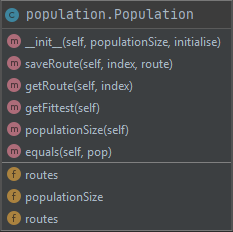
\includegraphics[scale=0.8]{images/population.png}
	\caption{Population osztály elemei}
	\label{fig:population}
\end{figure}

Tartalmaz egy inicializáló metódust, ezen felül itt kapott helyet az út mentése, kiolvasása is. A legfitebb érték meghatározásán kívűl a populációk összehasonlításával is foglalkozik az oszály. 

\subsection{A \texttt{Route} osztály}

Az optimális út kiszámításához használt osztály (\ref{fig:route}. ábra). Az alapvető inicializáláson kívűl jelen vannak még a helyes út kiszámításához használatos metódosok. Végezetül egy szövegformázó metódus is itt kapott helyet.

\begin{figure}[!htb]
	\centering
	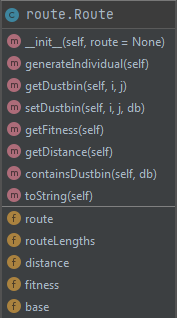
\includegraphics[scale=0.8]{images/route.png}
	\caption{A \texttt{Route} osztály elemei}
	\label{fig:route}
\end{figure}

\subsection{A \texttt{Routemanager} osztály}

Az oszály egyedeket kezel, három osztálymetódusból áll amik az optimális út eléréséhez nélkülözhetetlenek (\ref{fig:routeManager}. ábra).

\begin{figure}[!htb]
	\centering
	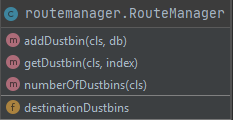
\includegraphics[scale=0.8]{images/routemanager.png}
	\caption{A \texttt{Routemanager} osztály elemei}
	\label{fig:routeManager}
\end{figure}

\Section{A megoldás tesztelése}

A genetikus algoritmus működését megvizsgáltam elitizmus használatával és a nélkül.
Ezek eredményeit a következő szakaszok foglalják össze.

\subsection{Elitizmus nélkül}

Az algoritmus paraméterei a következők voltak:
\begin{itemize}
\item A kiszállítási helyek száma: 40
\item Generációk száma: 40
\item Populáció nagysága: 20
\item Elitizmus: Hamis
\item  Futárok száma: 3
\end{itemize}

A futtatás eredményei \aref{fig:MTSPMultiDepo1}. és \ref{fig:MTSPMultiDepo1Route}. ábrán láthatók.

\begin{figure}[!htb]
\centering
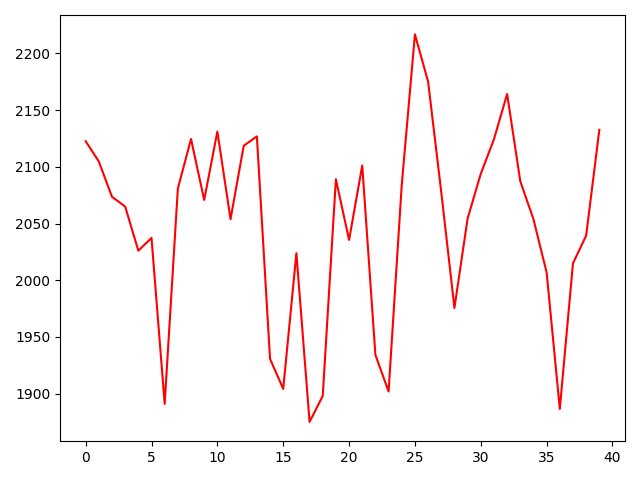
\includegraphics[scale=0.7]{images/MTSPMultiDepo1.png}
\caption{Fitnessz értékek generiónként elitizmus nélkül}
\label{fig:MTSPMultiDepo1}
\end{figure}

\begin{figure}[!htb]
\centering
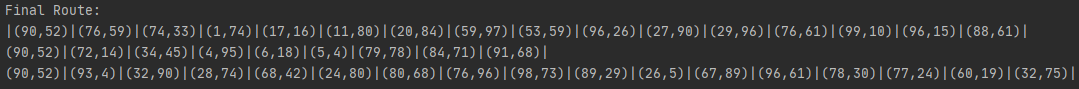
\includegraphics[width=\textwidth]{images/MTSPMultiDepo1Route.png}
\caption{Futárok útjai elitizmus nélkül}
\label{fig:MTSPMultiDepo1Route}
\end{figure}

\subsection{Elitizmussal}

Az előző paraméterezéssel, viszont elitizmus alkalmazásával \aref{fig:MTSPMultiDepo2}. és \ref{fig:MTSPMultiDepo2Route}. ábrákon látható eredményeket adta az algoritmus.

\begin{figure}[!htb]
\centering
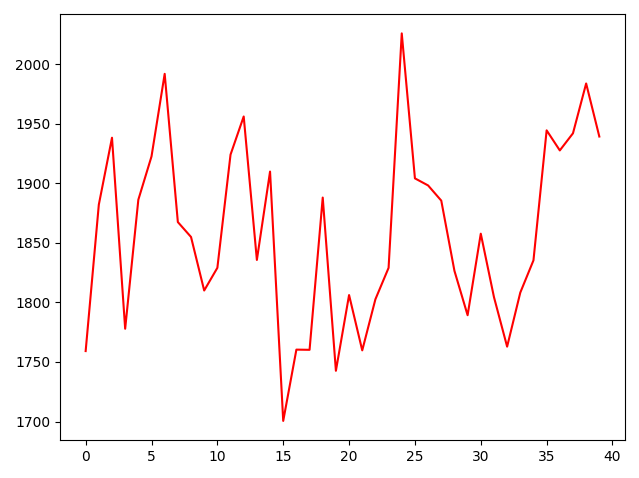
\includegraphics[scale=0.7]{images/MTSPMultiDepo2.png}
\caption{Fitnessz értékek generiónként elitizmussal}
\label{fig:MTSPMultiDepo2}
\end{figure}

\begin{figure}[!htb]
\centering
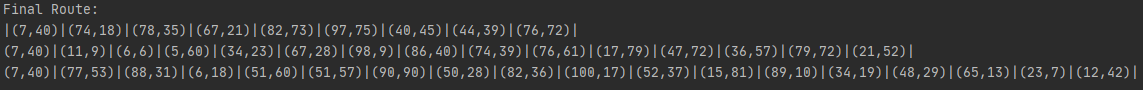
\includegraphics[width=\textwidth]{images/MTSPMultiDepo2Route.png}
\caption{Futárok útjai elitizmussal}
\label{fig:MTSPMultiDepo2Route}
\end{figure}
